
\section{The algorithm}
\label{sec:algorithm}

The algorithm we present is iterative. Each iteration is called \emph{era}. 

Each era $era_{i}$ is characterized by 
\begin{itemize}
\item the set of regions $\mathcal{R}_{i}$ in which the parameter space
$P_{1}\times\dots\times P_{n}$ is divided
\item its Pareto set $\mathscr{P}_{i}$
\item a set $test_{i}$ of at most $K$ configurations to evaluate
\end{itemize}
$K$ is a parameter that must be set before the algorithm runs.


\subsection{Start Condition}
$\mathcal{R}_{0}=\left\{ P_{1}\times\dots\times P_{n}\right\} $,
i.e. era $0$ has only one region that is the whole parameter space.
A random set $test_{0}$ of $K$ configurations is evaluated. The
Pareto set $\mathscr{P}_{0}=\mathscr{P}\left(test_{0}\right)$ is
calculated (see def \ref{pers02.def:Pareto-set} for the definition
of the operator $\mathscr{P}_{i}$ over a set)

\subsection{Iteration Rules}

For $era_{i}$ with $i>0$ the following operations must be performed.
\begin{enumerate}
\item \label{pers02.enu:K}For each region $R\in\mathcal{R}_{i}$, a set
$test_{R,i}$ of configurations is randomly chosen in%
\footnote{Therefore the chosen configurations can only be configurations of
$R$ not yet evaluated in past eras.%
} $R\setminus\bigcup_{j=0}^{i-1}test_{j}$. The number of configurations
in $test_{R,i}$ is set to%
\footnote{This means that $\frac{K}{\left|\mathcal{R}_{i}\right|}$ configurations
are to be chosen, but if not yet evaluated configurations in $R$
are less then $\frac{K}{\left|\mathcal{R}_{i}\right|}$, all of them
are chosen%
} 
\[
\min\left(\frac{K}{\left|\mathcal{R}_{i}\right|},\left|R\setminus\bigcup_{j=1}^{i-1}test_{j}\right|\right)
\]
The set 
\[
test_{i}=\bigcup_{R\in\mathcal{R}_{i}}test_{R,i}
\]
 is defined. 
\item All configurations on $test_{i}$ are simulated.
\item The Pareto set $\mathscr{P}_{i}$ for $era_{i}$ is defined as 
\[
\mathscr{P}_{i}=\mathscr{P}\left(test_{i}\cup\mathscr{P}_{i-1}\right)
\]

\item \label{pers02.enu:novelty_score_of_a_configuration}Every point $\mathbf{p}$
of%
\footnote{The innovation score is not given to those points in $test_{i}$ that
are not in the Pareto set%
} $test_{i}\cap\mathscr{P}_{i}$ is given an \emph{innovation score
}defined as:
\[
is\left(\mathbf{p}\right)=\min\left\{ \left.s\left(\mathbf{q}\rightarrow\mathbf{o}\left(\mathbf{p}\right)\right)\right|\mathbf{q}\in\mathscr{P}_{i-1}\right\} 
\]
 (a configuration $\mathbf{p}$ is characterized by as much innovation
as more separated it is from the configurations of the previous era)\@.
\item Every region $R\in\mathcal{R}_{i}$ is given an innovation score defined
as:
\[
is\left(R\right)=\sum\left\{ \left.is\left(\mathbf{p}\right)\right|\mathbf{p}\in\mathscr{P}_{i}\cap R\right\} 
\]

\item The total innovation score for the entire era is:
\[
is_{TOT,i}=\sum_{R\in\mathcal{R}_{i}}is\left(R\right)
\]

\item The average innovation score for the entire era is also calculated
as:
\[
is_{av,i}=\frac{is_{TOT,i}}{\left|\mathcal{R}_{i}\right|}
\]
where $\left|\mathcal{R}_{i}\right|$ is the number of regions of
era $i$ .
\item $\mathcal{R}_{i}$ is partitioned in three subsets (their meaning
will be discussed later):

\begin{enumerate}
\item high innovation regions 
\[
\mathcal{R}_{i,h}=\left\{ \left.R\in\mathcal{R}_{i}\right|is\left(R\right)>\alpha\cdot is_{av,i-1}\right\} 
\]
 where $\alpha$ is a constant defined by the designer (for example
$\alpha=1.2$). Each $R\in\mathcal{R}_{i,h}$ is split in $\mathcal{R}^{R}$
(as stated in def \ref{pers02.def:Splitting-a-region})
\item low innovation regions 
\[
\mathcal{R}_{i,l}=\left\{ \left.R\in\mathcal{R}_{i}\right|0<is\left(R\right)\le\alpha\cdot is_{av,i-1}\right\} 
\]
They are not changed.
\item no innovation regions 
\[
\mathcal{R}_{i,n}=\left\{ \left.R\in\mathcal{R}_{i}\right|is\left(R\right)=0\right\} 
\]
\end{enumerate}

\item Disjoint couples of contiguous regions $\left(R_{1},R_{2}\right)$,
with $R_{1},R_{2}\in\mathcal{R}_{i,n}$ are selected. The set of this
couples is indicated as $\mathcal{C}$. The couples of regions are
merged:
\[
\forall\left(R_{1},R_{2}\right)\in\mathcal{C}\Rightarrow R=R_{1}+R_{2}
\]
 (see def \ref{pers02.def:Merging-regions})
\item The set of regions $\mathcal{R}_{i+1}$ for the following era is defined
as:
\[
\mathcal{R}_{i+1}=
\]
\[
=\left(\bigcup_{R\in\mathcal{R}_{i,h}}\mathcal{R}^{R}\right)\cup\mathcal{R}_{i,l}\cup
\]
\[
\cup\left(\mathcal{R}_{i,n}\setminus\bigcup_{\left(R_{1},R_{2}\right)\in\mathcal{C}}\left\{ R_{1},R_{2}\right\} \right)\cup
\]
\[
\cup\left(\bigcup_{\left(R_{1},R_{2}\right)\in\mathcal{C}}\left(R_{1}+R_{2}\right)\right)
\]

\end{enumerate}

\subsection{Termination Condition}
The algorithm terminates at step $k$ if
\[
is_{TOT,k},is_{TOT,k-1},\dots,is_{TOT,k-\beta}\le\gamma\cdot is_{TOT,k-\left(\beta-1\right)}
\]
 where $\beta$ and $\gamma$ are selected by the experimenter (see
remark \ref{rem:termination}).
\begin{remark}
\label{pers02.rem:smaller_regions}The rule \ref{pers02.enu:K} of
the iteration rules says that the smaller is a region, the more ``crowded''
it is. It means that configurations in smaller regions are evaluated
with more ``attention'' (see figure \ref{pers02.fig:small_and_big}).

\begin{figure}[h]
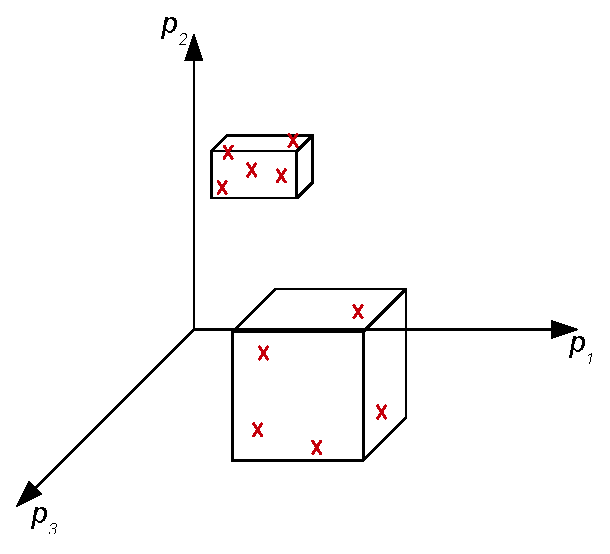
\includegraphics[width=0.5\columnwidth]{img/small_and_big}

\caption{\label{pers02.fig:small_and_big}In this example 5 configurations
are evaluated in a small region and in a bigger region. In can be
seen that smaller region is more crowded.}


\end{figure}

\end{remark}

\begin{remark}
The rule \ref{pers02.enu:novelty_score_of_a_configuration} says that
a configuration whose objectives are more ``separated'' by the previous
Pareto front, has to be taken in greater account than others. A configuration
that is very near, in the objective space, to the previous Pareto
front doesn't add a true innovation. Therefore, the innovation score
of a configuration is a measure of how much interest we have in considering
it (see figure \ref{pers02.fig:Novelty-score-of-a-config}).

\begin{figure}[h]
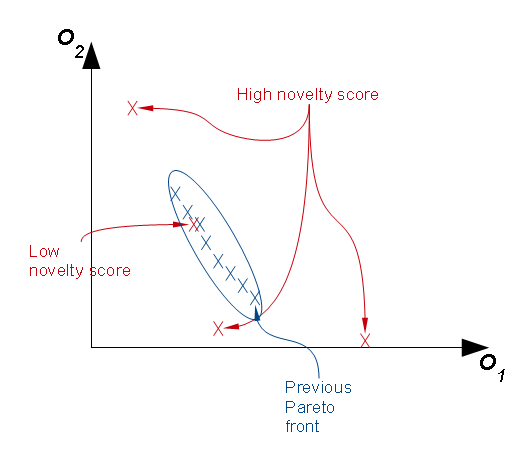
\includegraphics[width=0.5\columnwidth]{img/novelty_score}

\caption{\label{pers02.fig:Novelty-score-of-a-config}innovation score of a
configuration}


\end{figure}

\end{remark}

\begin{remark}
The innovation score of a region is a measure of how much different
are the points that it adds to Pareto Front compared to the previous
Pareto front. ``High innovation regions'' are the ones in which
more configurations are worth evaluating, because they add many points
on not yet well explored Pareto front areas. Therefore, these regions
are split in the next era (see remark \ref{pers02.rem:smaller_regions})
and more ``crowded'' by simulations. ``No innovation regions''
are the ones that have proved to add few points on Pareto fronts,
probably very near to previous Pareto front points and a Pareto front
point near to previous points is not so much interesting. Therefore
it's not worth evaluating many of their configurations and it is useful
to merge these regions, in order to less densely evaluate them.

%ULTERIORI GIUSTIFICAZIONI SULL'IMPORTANZA DI CONSIDERARE LA DIVERSITA'
%DELLE SOLUZIONI SI TROVA IN ext12.pag5 E ALTRI.

\end{remark}

\begin{remark}
\label{rem:termination}The algorithm terminates when in the last
$\beta$ iterations not a great ``amount of innovation'' has been
discovered. Therefore it is very probably that carrying on iterating
will not considerably change the Pareto front already formed. It's
not recommended to chose $\beta=1$, because it is possible that the
Pareto fronts $\mathbf{o}\left(\mathscr{P}_{k-1}\right)$ and $\mathbf{o}\left(\mathscr{P}_{k}\right)$
are not very different but next Pareto fronts could be. In other words,
it's unsafe to terminate as soon as the Pareto front doesn't change
enough between two consecutive eras, thus a strategy taking into
account the history of the Pareto fronts has been adopted in the
proposed approach.
\end{remark}
%!!! IN INGLESE E' PIU' CORRETTO DIRE: ``IT IS POSSIBLE THAT THE PARETO
%FRONTS WERE NOT VERY DIFFERENT''? (CON ``WERE'' AL POSTO DI ``ARE'')


\begin{remark}
Merging and splitting the regions are very dynamic processes. A portion
of the parameter space can be populated by a large number of small
regions in some eras, but can be covered by a small number of large
regions in next eras. This can be explained saying that, after a number
of eras of intense exploration of a portion of parameter space, this
exploration has turned to be enough thorough and so it was time for
other portions to be minutely scanned.
\end{remark}
